\chapter{O Método de Elementos Discretos} \label{ch:discrete_element_method}

\alert{Descrever aqui as características básicas e gerais que o \DEM{} possui}

O Método de Elementos Discretos (\DEM{}\footnote{Do inglês, \textit{Discrete Element Method}.}) refere-se a uma família de métodos numéricos aplicados na simulação de sistemas de partículas. Esses métodos compartilham diversas características entre si, como o monitoramento da vizinhança de cada partícula, o cálculo explícito das variáveis do problema a partir de seus valores nos instantes anteriores, dentre outras.

Este capítulo é dedicado à apresentação e à explicação dessas características. São apresentados o funcionamento geral de um algoritmo \DEM{}, o procedimento de solução das equações do problema e as principais etapas do método.

\alert{Talvez descrever melhor o que há em cada seção}

\section{Características Gerais do Método}

Segundo \citeonline[p. 1]{bib:bicanic2007}, o \DEM{} constitui-se de técnicas de modelagem computacional indicadas para a simulação do comportamento dinâmico de conjuntos de partículas de geometria arbitrária sujeitas a restrições de contato variantes no tempo.

Conforme a definição apresentada por \apudonline{bib:cundall1989}{bib:bicanic2007}, métodos de elementos discretos são métodos computacionais que:
\begin{alineas}
	\item consideram deslocamentos e rotações finitos de corpos discretos;
	\item reconhecem novos contatos automaticamente à medida que a simulação progride.
\end{alineas}

Cada partícula é considerada um corpo rígido com seis graus de liberdade: três translações e três rotações, e está sujeita às equações diferenciais de movimento descritas na \cref{sec:equations_of_motion}. O processo de simulação consiste na solução dessas equações. 

Em um sistema, porém, os elementos interagem entre si, e as forças e os torques atuantes sobre eles dependem dessas interações. Sendo assim, é necessário o \textit{monitoramento das vizinhanças}, isto é, o método deve sempre determinar quais são os pares de elementos que interagem em cada passo de tempo. Dentre os algoritmos disponíveis, destacam-se o algoritmo de Verlet, dedicado a partículas esféricas, o algoritmo \textit{link cell} e o algoritmo \textit{lattice}. \alert{São esses mesmo que considero depois?}

Os elementos da simulação ainda podem pertencer a \textit{tipos} distintos. Por exemplo, é possível distinguirem-se \textit{partículas}, elementos cujas equações de movimento precisam ser resolvidas, de \textit{elementos de contorno}, que têm seu estado conhecido já na etapa de inicialização do algoritmo. Além dos elementos de contorno, outras \textit{condições de contorno} podem ser aplicadas ao sistema, como restrições de movimento, paredes reflexivas e condição de repetição.

De acordo com \citeonline[p. 2]{bib:bicanic2007}, existem diversas metodologias para a simulação com elementos discretos, sendo que as variações ocorrem:
\begin{alineas}
	\item nos algoritmos de detecção de contatos;
	\item nas formulações para as interações;
	\item nas condições de contorno;
	\item na consideração de modelos de fratura, fragmentação ou aglutinação;
	\item nos métodos de integração das equações;
	\item nos algoritmos de monitoramento de vizinhanças.
\end{alineas}

\subsection{Discretização Temporal}

Como é recorrente em métodos de simulação numérica, o \DEM{} conta com a discretização do tempo para a solução das equações de movimento. Para o intervalo de simulação \(\interval{\initialInstant}{\finalInstant}\), sendo \(\initialInstant\) o instante inicial e \(\finalInstant\), o final, uma discretização temporal é um conjunto \(\set{t_0, t_1, \dotsc, t_{\numberOfTimesteps}}\) tal que
\begin{equation*}
	\initialInstant = \instant[0] < \instant[1] < \dotsb < \instant[\numberOfTimesteps - 1] < \instant[\numberOfTimesteps] = \finalInstant.
\end{equation*}

O valor \(\numberOfTimesteps\) é o número de passos de tempo da simulação. Um passo de tempo é o período compreendido entre dois instantes consecutivos da discretização. A duração do \(n\)-ésimo passo de tempo é dada então por
\begin{equation*}
	\Dt[n] \eqdef \instant[n] - \instant[n-1],
\end{equation*}
e escreve-se \(\Dt\) no caso em que os passos de tempo têm todos a mesma duração.

Com isso, o objetivo do Método de Elementos Discretos torna-se obter a solução para as coordenadas das partículas no tempo discretizado.

\subsection{Solução das Equações}

A solução das equações governantes do sistema é feita conforme explicado na \cref{subsec:motion_equations_solution} utilizando algoritmos de integração como o algoritmo de Gear, descrito na \cref{sec:gear_integration_scheme}.

Uma característica dos métodos de elementos discretos tradicionais é serem métodos explícitos, ou seja, o estado do sistema de partículas no instante \(\instant[n]\) é calculado a partir do estado em \(\instant[n-1]\) que se supõe ser conhecido. Isso é evidente no algoritmo de Gear.

O procedimento de solução das equações é apresentado em maiores detalhes na \cref{subsec:simulation:equation_solution}.

\subsection{Elementos da Simulação}

A classificação dos elementos pertencentes à simulação tem a finalidade de possibilitar simplificações, de determinar os métodos de busca de vizinhança, de busca de contato e de integração das equações, e de reduzir o custo computacional do algoritmo.

Não existe uma classificação comum a todos os métodos de elementos discretos, mas podem se observar diferenciações baseadas na geometria, nas propriedades, na forma como as coordenadas são obtidas e nas restrições aplicadas. 

Toda simulação possui um \textit{conjunto universo} \(\universeSet\) que contém todas as entidades consideradas pelo algoritmo: corpos, fluidos, campos de força, entre outras. Nos métodos de elementos discretos, os corpos rígidos pertencentes ao conjunto universo são agrupados no \textit{conjunto de elementos} \(\elementSet\). Por fim, é possível dividir-se o conjunto de elementos em um \textit{conjunto de partículas} \(\particleSet\) e um \textit{conjunto de elementos de contorno} \(\boundarySet\).

O conjunto de partículas é o conjunto de todos os elementos para os quais as equações de movimento devem ser resolvidas. Essa resolução é feita de acordo com os algoritmos de integração. 

Os elementos de contorno, por outro lado, são elementos cujos estados já são conhecidos como funções explícitas do tempo desde a etapa de inicialização. Exemplo disso são os elementos fixos, cujas coordenadas são sempre iguais às coordenadas iniciais. Elementos de contorno, portanto, representam um alívio do custo computacional, pois não é necessária a resolução de suas equações de movimento, embora ainda sejam necessários no cálculo das interações com as partículas. Uma função que determine completamente um elemento em cada instante de tempo é chamada de \textit{função de evolução}.

Campos de força, em geral, são considerados como entidades externas ao domínio da simulação, atuando indistintamente sobre todas as partículas do sistema e contribuindo com parcelas das forças externas \(\external\forcei\) e dos torques externos \(\external\torquei\).

Outras características que podem ser atribuídas aos elementos da simulação são:
\begin{alineas}
\item \textit{Propriedades:} as propriedades que se atribuem aos elementos são essenciais para o cálculo das interações que ocorrem entre eles. Seus valores podem ser função do material de que os corpos são compostos, de parâmetros obtidos experimentalmente, entre outros. Exemplos de propriedades físicas são a massa específica e o módulo de elasticidade. Além disso, outros parâmetros podem ser atribuídos às partículas, como o coeficiente de atrito e o amortecimento, de acordo com a \cref{sec:collision_force_models}.

\begin{figure}[h]
	\caption{Formas geométricas mais aplicadas nos métodos de elementos discretos.}
	% \vspace{-0.5cm}
	\centering
	\captionsetup[subfloat]{labelfont=bf}
	\subfloat{
		\centering
		\begin{subfigure}[t]{\smallresultsfigwidth}
			\centering
			\alert{Figura aqui (partícula esférica)}
			\caption{Geometria esférica.}
			\label{subfig:element_geometry:sphere}
		\end{subfigure}
		\begin{subfigure}[t]{\smallresultsfigwidth}
			\centering
			\alert{Figura aqui (elemento plano)}
			\caption{Geometria plana.}
			\label{subfig:element_geometry:plane}
		\end{subfigure}
		\begin{subfigure}[t]{\smallresultsfigwidth}
			\centering
			\alert{Figura aqui (superelipsoide)}
			\caption{Geometria superelipsoidal.}
			\label{subfig:element_geometry:ellipsoid}
		\end{subfigure}
		\begin{subfigure}[t]{\smallresultsfigwidth}
			\centering
			\alert{Figura aqui (poliedro)}
			\caption{Geometria poliédrica.}
			\label{subfig:element_geometry:polyhedron}
		\end{subfigure}
		\begin{subfigure}[t]{\smallresultsfigwidth}
			\centering
			\alert{Figura aqui (partícula composta)}
			\caption{Geometria composta.}
			\label{subfig:element_geometry:composite_particle}
		\end{subfigure}
	}
	% {\centerline{\includegraphics[scale=#2]{#1}}}
	% \vspace{-0.2cm}
	\label{fig:element_geometry}
	\sourceMe
	% \vspace{-1cm}
\end{figure}

\item \textit{Geometria:} a geometria dos elementos determina fundamentalmente os modelos de interação a que os elementos são submetidos, os métodos de monitoramento de vizinhança e a busca por contatos. As geometrias mais simples, nas quais este trabalho se baseia, são a esférica e a plana. Também são aplicáveis superelipsoides e poliedros, e formas geométricas arbitrariamente mais complexas podem ser obtidas através da composição de partículas de forma mais simples. Um exemplo da aplicação de superelipsoides pode ser encontrado em \citeonline{bib:sampaio}. Essas formas estão representadas na \cref{fig:element_geometry}.

\item \textit{Restrição de movimento:} o tipo de restrição de movimento que um elemento sofre também pode ser considerado. É usual definirem-se elementos \textit{fixos}, cujas coordenadas se mantêm constantes na simulação, e elementos com movimento \textit{prescrito}, que são aqueles cujas coordenadas são definidas por funções temporais arbitrárias fornecidas na etapa de inicialização. Outra restrição bastante aplicada é aquela que ocorre entre os subelementos de uma partícula composta, limitando o seu movimento relativo. Mais detalhes sobre essa restrição podem ser encontrados em \citeonline{bib:computational_granular_dynamics}.
\end{alineas}

\subsection{Algoritmo Geral do \DEM{}} \label{sec:dem_algorithm}

De forma geral, os métodos de elementos discretos apresentam um algoritmo básico \alert{não gostei dessa frase}. Esse algoritmo é composto, essencialmente, da etapa de inicialização, do laço de simulação e da terminação do programa.

O laço da simulação é a parte mais custosa do algoritmo pois é nele que ocorrem as subetapas de resolução das equações e exportação de dados.

A forma geral desse algoritmo pode ser representada como o fluxograma exposto na \cref{fig:general_algorithm}.

\begin{figure}[h]
	\caption{Floxugrama do funcionamento geral do \DEM{}.}
	% \vspace{-0.5cm}
	\centering
		\alert{Colocar imagem representando o \DEM{}}
		% 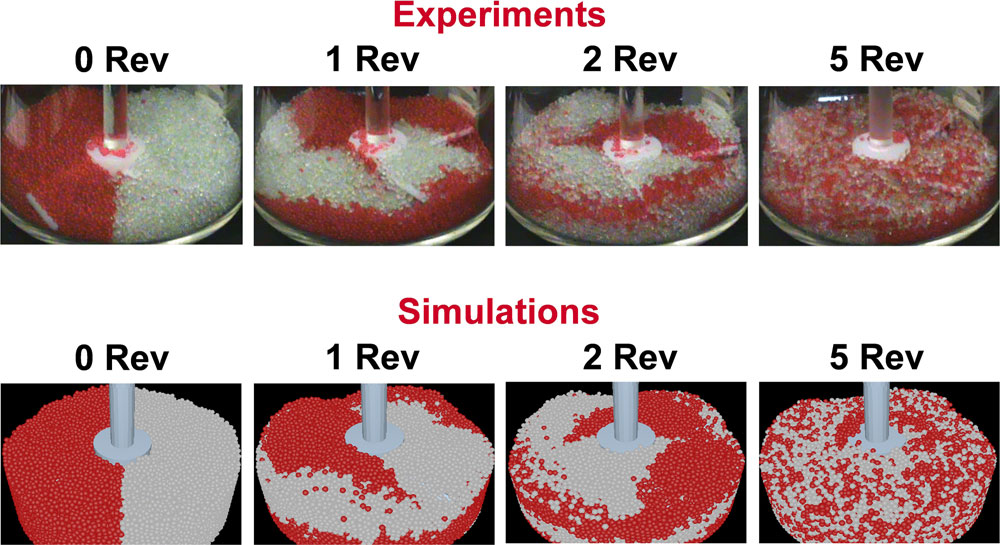
\includegraphics[width=0.65\textwidth]{images/introduction/drug_production.png}
	% {\centerline{\includegraphics[scale=#2]{#1}}}
	% \vspace{-0.2cm}
	\label{fig:general_algorithm}
	\source{\alert{Citar fonte}}
	% \vspace{-1cm}
\end{figure}

As etapas do \DEM{} são apresentadas em mais detalhes na \cref{sec:algorithm_steps}.

\section{Etapas do Algoritmo} \label{sec:algorithm_steps}
\subsection{Inicialização do Sistema de Partículas}

A primeira etapa em uma simulação \DEM{} é a inicialização do sistema de partículas. Essa etapa consiste em se definir o ambiente da simulação e se construírem todos os elementos necessários.

De acordo com \citeonline{bib:computational_granular_dynamics}, a inicialização geralmente é feita por meio de um arquivo de entrada, muito embora \textit{softwares} de simulação geralmente apresentem uma interface gráfica com essa finalidade. 

O resultado dessa etapa é o estado inicial do sistema de partículas, com todas as posições, orientações e outras variáveis inicializadas. Os parâmetros de entrada são:
\begin{alineas}
\item \textit{Parâmetros da simulação:} os principais parâmetros, como instantes inicial e final, passo de tempo, critério de parada e caminhos para exportação de arquivos, são configurados;
\item \textit{Partículas:} todas as partículas do sistema devem ser construídas. A cada partícula deve ser atribuída um vetor posição, uma orientação e propriedades físicas iniciais. Além disso, as derivadas dos vetores posição e orientação devem ser informados. A geometria das partículas também deve ser definida;
\item \textit{Elementos de contorno:} de maneira semelhante às partículas, os elementos de contorno devem ser construídos com geometria, posição, orientação e propriedades físicas. Ainda, é necessário determinar-se a função de evolução desses elementos;
\item \textit{Outras entidades:} todas as outras entidades do sistema, como campos de força e fluidos, também devem ser inicializadas;
\item \textit{Interações:} além dos elementos do sistema, devem ser definidos os modelos de interação utilizados. Por exemplo, para as forças normais de colisão entre partículas esféricas, deve-se escolher entre o modelo de amortecimento linear, o de esferas viscoelásticas ou outros que estejam implementados no simulador;
\item \textit{Algoritmo de integração:} a determinação do algoritmo de solução das equações do sistema é fundamental para a simulação. Dentre os principais métodos aplicados se encontram aqueles citados na \cref{subsec:motion_equations_solution}: o algoritmo de Gear, o método \textit{leapfrog}, os métodos de Verlet e os de Runge-Kutta, desde que estejam disponíveis no simulador;
\item \textit{Método de monitoramento de vizinhanças:} a escolha do método de monitoramento de vizinhanças também é de extrema importância na simulação. Esse método tem por finalidade determinar quais elementos interagem em cada passo de tempo, sendo determinante para o custo computacional do algoritmo. O monitoramento de vizinhanças deve ser escolhido tendo em vista os tipos e as formas geométricas dos elementos considerados e as características da simulação;
\item \textit{Outros parâmetros:} por fim, dependendo da implementação do simulador e do método de elementos discretos usado, podem ser necessários outras entradas mais específicas, além das já citadas.
\end{alineas}

\alert{O seguinte deve ser movido se houver um capítulo para implementação computacional:}

Neste trabalho, foi utilizado o formato \JSON{} para os arquivos de entrada. O \JSON{} é um formato de arquivo independente de linguagem que facilita a troca de informações, sendo desenhado para ser facilmente lido por humanos e interpretado por programas de computador \cite{bib:json}. Como exemplo, é apresentado, no \cref{app:code_listings}, o arquivo de inicialização do problema de lançamento oblíquo, descrito na \cref{sec:free_fall}.

\subsection{Solução das Equações} \label{subsec:simulation:equation_solution}

De acordo com \citeonline{bib:computational_granular_dynamics}, a solução das equações pode ser dividida em quatro etapas, sendo elas:

% \begin{enumdesc}
% 	\item[Determinação da Vizinhança:] Nessa etapa, a vizinhança de cada partícula do sistema é construída (no primeiro instante) ou atualizada (em instantes posteriores da simulação). O objetivo é limitar a quantidade de interações avaliadas no passo de tempo. 
% 	\item[Predição:] Nesse passo, o estado do sistema no instante \(\instant[n]\) é predito em função do estado em \(\instant[n-1]\). Essa predição é feita por métodos de extrapolação, como explicado na \cref{subsec:prediction}. \label{item:DEM_prediction}
% 	\item[Interação:] A partir do estado predito do sistema, são computadas as interações entre cada partícula e os elementos de sua vizinhança. \label{item:DEM_interaction}
% 	\item[Correção:] Na etapa de correção, o estado do sistema no instante \(\instant[n]\) é corrigido em função das interações calculadas na etapa \ref{item:DEM_interaction} e das equações governantes do problema, como apresentado na \cref{subsec:correction}. Embora esse processo não seja exato, o DEM considera o estado corrigido como a solução do problema para o instante \(\instant[n]\). \label{item:DEM_correction}
% \end{enumdesc}
\begin{enumerate}
	\item \textit{Determinação da Vizinhança:} Nessa etapa, a vizinhança de cada partícula do sistema é construída (no início da simulação) ou atualizada (em instantes posteriores) com o intuito de limitar a quantidade de interações avaliadas no passo de tempo. \label{item:DEM_neighborhood}
	\item \textit{Predição:} Nesse passo, o estado do sistema no instante \(\instant[n]\) é predito em função do estado em \(\instant[n-1]\) por meio de métodos de extrapolação, como explicado na \cref{subsec:prediction}. \label{item:DEM_prediction}
	\item \textit{Interação:} A partir do estado predito do sistema, são computadas as interações entre cada partícula e os elementos de sua vizinhança. \label{item:DEM_interaction}
	\item \textit{Correção:} Na etapa de correção, o estado do sistema no instante \(\instant[n]\) é corrigido em função das interações calculadas na etapa \ref{item:DEM_interaction} e das equações governantes do problema, como apresentado na \cref{subsec:correction}. Embora esse processo não seja exato, o DEM considera o estado corrigido como a solução do problema para o instante \(\instant[n]\). \label{item:DEM_correction}
\end{enumerate}

Os passos \ref{item:DEM_prediction}, \ref{item:DEM_interaction} e \ref{item:DEM_correction} são específicos do algoritmo de Gear, podendo mudar se forem adotados outros métodos.

Para a determinação da vizinhança no passo \ref{item:DEM_neighborhood}, são usados algoritmos de monitoramento de vizinhança, como explicado na \cref{sec:neighborhood}. O objetivo desta seção é, assim, apresentar os passos \ref{item:DEM_prediction}, \ref{item:DEM_interaction} e \ref{item:DEM_correction}, mostrando a aplicação dos conceitos apresentados no \cref{ch:mathematical_model} aos sistemas de partículas.

% \alert{é estranho colocar a vizinhança antes. Três motivos por que isso é feito: 1) a referência faz; 2) o passo de tempo que usamos é pequeno; 3) permite uma fácil alteração do algoritmo de integração da equação}

Para tanto, pode ser feita uma distinção entre o caso de partículas com geometria arbitrária, em que é necessário monitorar-se a orientação das partículas, e o de partículas esféricas, situação em que é possível aplicarem-se simplificações.

\subsubsection*{Caso Geral}

No caso de partículas quaisquer, o algoritmo de Gear precisa levar em consideração as parametrizações para as orientações das partículas.

Sendo \(\instant[n]\) o instante de interesse e \(\instant[n-1]\), o instante anterior em que o sistema é conhecido, as posições e as orientações das partículas podem ser previstas como na \cref{eq:prediction}. Escolhida uma ordem de extrapolação \(\taylorOrder\), e definido o conjunto \(\particleSet\) de partículas do sistema, calculam-se
\begin{equation*}
	\def\arraystretch{1.5}
	\begin{array}{c}
		\drvec{\taylorOrder}{\positionipr}\pqty{\instant[n]} = \extrapolationMatrix{\taylorOrder}[\Dt[n]]\cdot\drvec{\taylorOrder}{\positioni}\pqty{\instant[n-1]} \\
		\drvec{\taylorOrder}{\orientationipr}\pqty{\instant[n]} = \extrapolationMatrix{\taylorOrder}[\Dt[n]]\cdot\drvec{\taylorOrder}{\orientationi}\pqty{\instant[n-1]} \\
	\end{array}, \quad \particlei \in \particleSet,
\end{equation*}
em que \(\extrapolationMatrix{\taylorOrder}[\Dt[n]]\) é a matriz de extrapolação por expansão de Taylor de ordem \(\taylorOrder\) calculada com o passo de tempo \(\Dt[n]\), como indicada na \cref{subsec:prediction}.

A vizinhança de uma partícula, como explicado na \cref{sec:neighborhood}, é o conjunto de todas as entidades da simulação com as quais ela interage. A vizinhança da \(i\)-ésima partícula do sistema é denotada por \(\neighborhoodi\) \alert{Verificar se essas coisas já não foram ditas antes com a mudança das seções.}. Cada elemento \(\elementj\) da vizinhança de \(\particlei\) contribui para a força \(\forcei\) e o torque \(\torquei\) resultantes sobre a mesma com parcelas \(\forceji\) e \(\torqueji\) que são, por hipótese, dependentes apenas do par \(\orderedPair{\particlei}{\elementj}\), isto é,
\begin{equation*}
	\def\arraystretch{1.5}
	\begin{array}{c}
		\displaystyle \forceji \equiv \forceji\pqty{\particlei, \elementj} \\
		\displaystyle \torqueji \equiv \torqueji\pqty{\particlei, \elementj} \\
	\end{array}, \quad \particlei \in \particleSet, \elementj \in \neighborhoodi.
\end{equation*}

Mais ainda, a partícula \(i\) pode sofrer com forças e torques provocados por entidades externas ao sistema, como forças de campo, cujas resultantes são dadas por
\begin{equation*}
	\def\arraystretch{1.5}
	\begin{array}{c}
		\external\forcei \equiv \external\forcei\pqty{\particlei} \\
		\external\torquei \equiv \external\torquei\pqty{\particlei} \\
	\end{array}, \quad \particlei \in \particleSet.
\end{equation*}
 
Com isso, obtêm-se os vetores resultantes de acordo com o princípio da superposição dado pelas \namecrefs{eq:superposition_translation} \labelcref{eq:superposition_translation,eq:superposition_rotation}:
\begin{equation*}
	\def\arraystretch{1.5}
	\begin{array}{c}
		\resultingForcei = \dsum_{\elementj\in\neighborhoodi}\forceji + \external\forcei\\
		\resultingTorquei = \dsum_{\elementj\in\neighborhoodi}\torqueji + \external\torquei
	\end{array}, \quad \particlei\in\particleSet.
\end{equation*}

A cada um dos graus de liberdade da partícula é associada uma equação que determina seu comportamento, e o algoritmo de Gear baseia-se nisso para executar a etapa de correção. As equações de movimento \eqref{eq:motion_first} e \eqref{eq:diff_equation_orientation_parametrization}, então, são utilizadas para se corrigirem as derivadas de segunda ordem da posição e da orientação das partículas:
\begin{equation*}
	\def\arraystretch{1.5}
	\begin{array}{c}
		\displaystyle \accelerationicorr =  \dfrac{1}{\massi}\cdot \forcei \\
		\displaystyle \dorientationicorr{2} = \eqFor{\orientationScalar}\pqty{\torquei, \orientationipr, \dorientationipr{1}}
	\end{array}, \quad \particlei \in \particleSet,
\end{equation*}
sendo que \(\eqFor{\orientationScalar}\) depende da parametrização escolhida para a orientação.

Definem-se, então, os erros
\begin{equation*}
	\def\arraystretch{1.5}
	\begin{array}{c}
		\Delta \accelerationi\pqty{\instant[n]} = \accelerationicorr\pqty{\instant[n]} - \accelerationipr\pqty{\instant[n]} \\
		\Delta \dorientationi{2}\pqty{\instant[n]} = \dorientationicorr{2}\pqty{\instant[n]} - \dorientationipr{2}\pqty{\instant[n]} \\
	\end{array}, \quad \particlei\in\particleSet.
\end{equation*}

Por fim, resta executar a correção nos vetores de derivadas. Tanto para a translação quanto para a rotação, a equação diferencial é de ordem \(\eqOrder = 2\), e isso, juntamente com a ordem de extrapolação \(\taylorOrder\), determina as constantes de correção. Com isso, utiliza-se a equação \eqref{eq:correction_simplified} para se escrever	
\begin{equation*}
	\def\arraystretch{1.5}
	\begin{array}{l}
		\drvec{\taylorOrder}{\positionicorr}\pqty{\instant[n]} = \drvec{\taylorOrder}{\positionipr}\pqty{\instant[n]} + \correctorConstantVector{\taylorOrder}{2}\cdot\dfrac{\Dt[n]^2}{2}\Delta \accelerationi\pqty{\instant[n]} \\
		\drvec{\taylorOrder}{\orientationicorr}\pqty{\instant[n]} = \drvec{\taylorOrder}{\orientationipr}\pqty{\instant[n]} + \correctorConstantVector{\taylorOrder}{2}\cdot\dfrac{\Dt[n]^2}{2}\Delta \dorientationi{2}\pqty{\instant[n]}
	\end{array}, \quad \particlei\in\particleSet.
\end{equation*}

Dessa forma, estão calculadas a posição, a orientação e as suas derivadas, e o instante de tempo \(\instant[n]\) é considerado solucionado.

\alert{O seguinte deve ser movido, ou alterado para o caso de partículas esféricas, caso exista um capítulo para implementação computacional.}

Esse procedimento pode ser representado em forma de pseudocódigo como na \cref{lst:equations_solution}.
\begin{lstlisting}[float, floatplacement=h, language=pseudocode, label=lst:equations_solution, caption=Pseudocódigo para a solução das equações de movimento por meio do algoritmo de Gear.]
// Algoritmo de Gear
para cada partícula $\particlei \in \particleSet$:
(*\indentrule*)	// Determinação da Vizinhança
(*\indentrule*)	determinar a vizinhança $\neighborhoodi$
(*\indentrule*)	// Predição
(*\indentrule*)	calcular o vetor posição predito $\drvec{\taylorOrder}{\positionipr}\pqty{\instant[n]} = \extrapolationMatrix{\taylorOrder}[\Dt[n]]\cdot\drvec{\taylorOrder}{\positioni}\pqty{\instant[n-1]}$
(*\indentrule*)	calcular o vetor orientação predito $\drvec{\taylorOrder}{\orientationipr}\pqty{\instant[n]} = \extrapolationMatrix{\taylorOrder}[\Dt[n]]\cdot\drvec{\taylorOrder}{\orientationi}\pqty{\instant[n-1]}$
(*\indentrule*)	atribuir $\resultingForcei \gets \nullVector$
(*\indentrule*)	atribuir $\resultingTorquei \gets \nullVector$

para cada partícula $\particlei \in \particleSet$:
(*\indentrule*)	// Interação (*\label{lstline:interaction_begin}*)
(*\indentrule*)	para cada elemento $\elementj \in \neighborhoodi$:
(*\indentrule*)	(*\indentrule*)	calcular a força$$ $\forceji$ que $\elementj$ aplica sobre $\particlei$
(*\indentrule*)	(*\indentrule*)	calcular o torque$$ $\torqueji$ que $\elementj$ aplica sobre $\particlei$
(*\indentrule*)	(*\indentrule*)	adicionar $\resultingForcei \gets \resultingForcei + \forceji$
(*\indentrule*)	(*\indentrule*)	adicionar $\resultingTorquei \gets \resultingTorquei + \torqueji$
(*\indentrule*)	fim (*\label{lstline:particle_element_interaction_end}*)
(*\indentrule*)	para cada entidade $\element$ externa ao domínio:
(*\indentrule*)	(*\indentrule*)	calcular a componente de força$$ $\force$ que $\element$ aplica sobre $\particlei$
(*\indentrule*)	(*\indentrule*)	calcular a componente de torque$$ $\torque$ que $\element$ aplica sobre $\particlei$
(*\indentrule*)	(*\indentrule*)	adicionar $\resultingForcei \gets \resultingForcei + \force$
(*\indentrule*)	(*\indentrule*)	adicionar $\resultingTorquei \gets \resultingTorquei + \torque$
(*\indentrule*)	fim
(*\indentrule*)
(*\indentrule*)	// Correção
(*\indentrule*)	calcular o valor corrigido $\accelerationicorr =  \dfrac{1}{\massi}\cdot \forcei$
(*\indentrule*)	calcular o valor corrigido $\dorientationicorr{2} = \eqFor{\orientationScalar}\pqty{\torquei, \orientationipr, \dorientationipr{1}}$
(*\indentrule*)	calcular o erro $\Delta \accelerationi\pqty{\instant[n]} = \accelerationicorr\pqty{\instant[n]} - \accelerationipr\pqty{\instant[n]}$
(*\indentrule*)	calcular o erro $\Delta \dorientationi{2}\pqty{\instant[n]} = \dorientationicorr{2}\pqty{\instant[n]} - \dorientationipr{2}\pqty{\instant[n]}$
(*\indentrule*)	corrigir o vetor posição $\drvec{\taylorOrder}{\positionicorr}\pqty{\instant[n]} = \drvec{\taylorOrder}{\positionipr}\pqty{\instant[n]} + \correctorConstantVector{\taylorOrder}{2}\cdot\dfrac{\Dt[n]^2}{2}\Delta \accelerationi\pqty{\instant[n]}$
(*\indentrule*)	corrigir o vetor orientação $\drvec{\taylorOrder}{\orientationicorr}\pqty{\instant[n]} = \drvec{\taylorOrder}{\orientationipr}\pqty{\instant[n]} + \correctorConstantVector{\taylorOrder}{2}\cdot\dfrac{\Dt[n]^2}{2}\Delta \dorientationi{2}\pqty{\instant[n]}$
(*\indentrule*)	atribuir $\drvec{\taylorOrder}{\position}\pqty{\instant[n]} \gets \drvec{\taylorOrder}{\positionicorr}\pqty{\instant[n]}$	// Dessa forma, a correção é(**) considerada exata
(*\indentrule*)	atribuir $\drvec{\taylorOrder}{\orientation}\pqty{\instant[n]} \gets \drvec{\taylorOrder}{\orientationicorr}\pqty{\instant[n]}$	//		
fim
\end{lstlisting}
\alert{Usar o código para partículas quaisquer ou apenas para as esféricas?}

\subsubsection*{Partículas Esféricas}

Para partículas esféricas, as equações de movimento assumem uma forma mais simples, conforme mostrado na \autoref{subsubsec:rotation_of_spherical_particles}. 

Novamente, o algoritmo inicia com a escolha da ordem de derivação \(\taylorOrder\) para a predição conforme a equação \eqref{eq:prediction}. Dessa vez, porém, a velocidade angular é prevista com uma ordem a menos que a posição.
\begin{equation*}
	\def\arraystretch{1.5}
	\begin{array}{c}
		\drvec{\taylorOrder}{\positionipr}\pqty{\instant[n]} = \extrapolationMatrix{\taylorOrder}[\Dt[n]]\cdot\drvec{\taylorOrder}{\positioni}\pqty{\instant[n-1]} \\
		\drvec{\taylorOrder-1}{\angularVelocityipr}\pqty{\instant[n]} = \extrapolationMatrix{\taylorOrder-1}[\Dt[n]]\cdot\drvec{\taylorOrder-1}{\angularVelocityi}\pqty{\instant[n-1]} \\
	\end{array}, \quad \particlei\in\particleSet.
\end{equation*}

O cálculo de forças e torques se dá de maneira idêntica ao caso geral, isto é,
\begin{equation*}
	\def\arraystretch{1.5}
	\begin{array}{c}
		\resultingForcei = \dsum_{\elementj\in\neighborhoodi}\forceji\pqty{\particlei, \elementj} + \external\forcei\pqty{\particlei}\\
		\resultingTorquei = \dsum_{\elementj\in\neighborhoodi}\torqueji\pqty{\particlei, \elementj} + \external\torquei\pqty{\particlei}
	\end{array}, \quad \particlei\in\particleSet.
\end{equation*}

E, como no caso geral, o valor corrigido para a aceleração advém da equação \eqref{eq:motion_first}:
\begin{equation*}
	\accelerationicorr\pqty{\instant[n]} = \dfrac{1}{\massi}\cdot\resultingForcei\pqty{\instant[n]}, \quad\particlei\in\particleSet.
\end{equation*}

Já para a aceleração angular, usa-se a equação de movimento rotacional simplificada para o caso de esferas \eqref{eq:rotation_spherical_particle}, obtendo-se, para cada \(\particlei\in\particleSet\),
\begin{equation*}
	\dangularVelocityicorr{1}\pqty{\instant[n]} = \dfrac{1}{\momentOfInertiai}\cdot\resultingTorquei\pqty{\instant[n]}
\end{equation*}

Com isso, os erros são dados por
\begin{equation*}
	\def\arraystretch{1.5}
	\begin{array}{c}
		\Delta \accelerationi\pqty{\instant[n]} = \accelerationicorr\pqty{\instant[n]} - \accelerationipr\pqty{\instant[n]} \\
		\Delta \dangularVelocityi{1}\pqty{\instant[n]} = \dangularVelocityicorr{1}\pqty{\instant[n]} - \dangularVelocityipr{1}\pqty{\instant[n]} \\
	\end{array}, \quad\particlei\in\particleSet.
\end{equation*}

E, finalmente, são corrigidos os vetores de derivadas conforme a equação \eqref{eq:correction_simplified}. Para a translação, a equação diferencial é de ordem \(\eqOrder = 2\), e então
\begin{equation*}
	\drvec{\taylorOrder}{\positionicorr}\pqty{\instant[n]} = \drvecipr{\taylorOrder}{\position}\pqty{\instant[n]} + \correctorConstantVector{\taylorOrder}{2}\cdot\dfrac{\Dt[n]^2}{2}\Delta \accelerationi\pqty{\instant[n]}, \quad\particlei\in\particleSet.
\end{equation*}

A velocidade angular, por sua vez, está sujeita a uma equação diferencial de primeira ordem. O vetor de coeficientes \(\correctorConstantVector{\taylorOrder-1}{1}\), portanto, deve ser calculado para \(\eqOrder=1\). Nessas condições, o vetor de derivadas da velocidade angular fica
\begin{equation*}
		\drvec{\taylorOrder}{\angularVelocityicorr}\pqty{\instant[n]} = \drvec{\taylorOrder}{\angularVelocityipr}\pqty{\instant[n]} + \correctorConstantVector{\taylorOrder-1}{1}\cdot\Dt[n]\cdot\Delta \dangularVelocityi{1}\pqty{\instant[n]}, \quad\particlei\in\particleSet.
\end{equation*}

Esse algoritmo pode ser implementado de maneira semelhante ao exposto na \cref{lst:equations_solution}.

\subsection{Exportação de Dados}

A exportação de dados é a subetapa da simulação em que, de fato, são obtidos os resultados da simulação. A saída do programa é o conjunto de informações de interesse produzidas e exportadas pelo simulador. Essa exportação é, geralmente, direcionada para um ou mais arquivos de saída.

O pós-processamento dos resultados consiste em se processarem os dados exportados da simulação com a finalidade de se obterem as informações de interesse. Para tanto, utilizam-se gráficos, animações, tabelas e diversas outras técnicas de visualização de dados.

Existem dois fatores limitantes quanto à aquisição dos dados da simulação: o primeiro é a restrição da memória do computador. Geralmente, a quantidade de passos de tempo simulados e o número de elementos do sistema gera um volume de dados maior que a capacidade da memória. A segunda restrição é que o processo de escrita em disco é frequentemente uma operação lenta, reduzindo o desempenho do computador.\footnote{Por simplicidade, é utilizado aqui o termo \textit{memória} para referir-se unicamente à \textit{memória principal} do computador, comumente representada pela memória \RAM{} e pelos registradores. Por outro lado, o termo \textit{disco} é usado para referir-se à \textit{memória secundária}. Esse tipo de memória é geralmente representada pelas memórias não voláteis, como discos rígidos (\HD s), unidades de estado sólido (\SSD s) e discos de leitura ótica (\CD s e \DVD s).}

Uma solução comumente adotada é a definição de dois parâmetros: o \textit{número de passos de tempo para armazenamento} \(\stepsForStoring\) e o \textit{número de passos armazenados para a escrita} \(\storagesForWriting\). O número \(\stepsForStoring\) conta quantos passos de tempo são simulados até que um seja armazenado. Com isso, a cada \(\stepsForStoring\) simulados, \(\stepsForStoring-1\) são descartados e apenas um é guardado na memória. O segundo parâmetro, \(\storagesForWriting\), define quantos passos de tempo são armazenados na memória antes de serem escritos em disco.

Essa solução pode ser implementada como na \cref{lst:data_exportation}. Definem-se os contadores \(\stepsForStoringCounter\) e \(\storagesForWritingCounter\), inicializados com o valor zero. A cada passo de tempo, o contador \(\stepsForStoringCounter\) é incrementado. Quando esse contador atinge o valor máximo de \(\stepsForStoring\), ele é reiniciado, o contador \(\storagesForWriting\) é incrementado e é feito um registro do instante de tempo na memória. Quando o contador \(\storagesForWritingCounter\) se iguala a \(\storagesForWriting\), o mesmo é reiniciado, e as informações armazenadas são escritas em disco.

\begin{lstlisting}[float, floatplacement=h, language=pseudocode, label=lst:data_exportation, caption=Pseudocódigo para a exportação de dados.]
inicializar $\stepsForStoringCounter \gets 0$
inicializar $\storagesForWritingCounter \gets 0$
// Laço de simulação 
enquanto o critério de parada não for atingido:
(*\indentrule*)	incrementar $\stepsForStoringCounter \gets \stepsForStoringCounter + 1$
(*\indentrule*)	se $\stepsForStoringCounter = \stepsForStoring$:
(*\indentrule*)	(*\indentrule*)	atribuir $\stepsForStoringCounter \gets 0$
(*\indentrule*)	(*\indentrule*)	incrementar $\storagesForWritingCounter \gets \storagesForWritingCounter + 1$
(*\indentrule*)	(*\indentrule*)	guardar estado atual na memória
(*\indentrule*)	(*\indentrule*)	se $\storagesForWritingCounter = \storagesForWriting$:
(*\indentrule*)	(*\indentrule*)	(*\indentrule*)	atribuir $\storagesForWritingCounter \gets 0$
(*\indentrule*)	(*\indentrule*)	(*\indentrule*)	escrever estados guardados nos arquivos de saída
(*\indentrule*)	(*\indentrule*)	fim 
(*\indentrule*)	fim
(*\indentrule*)	(*\hiddenCode*) // Solução das equações do sistema
fim
\end{lstlisting}

\subsection{Condição de Parada}

A condição de parada representa a condição que interrompe o laço de simulação e leva à finalização do programa. Essa condição se apresenta de diversas formas dependendo da aplicação, podendo levar em conta o estado do sistema e parâmetros da simulação \cite{bib:computational_granular_dynamics}. O critério de parada pode ser equivalentemente definido por um critério de continuação que, enquanto for verdadeiro, mantém a execução do laço.

Uma das condições mais simples e mais aplicadas é a condição de parada por tempo final da simulação. Esse critério baseia-se na definição de um valor \(\finalInstant\) para o instante final da simulação, e a simulação progride até que esse limite seja ultrapassado. O laço da simulação pode então ser representado como na \cref{lst:stop_criterion}. O instante inicial \(\initialInstant\) é proveniente da etapa de inicialização, e o \(n\)-ésimo passo de tempo \(\Dt[n]\) é dependente do método escolhido, do arquivo de inicialização e dos algoritmos de integração e de determinação de vizinhanças. \alert{Mover caso haja um capítulo próprio para implementação computacional.}

\begin{lstlisting}[float, floatplacement=h, language=pseudocode, label=lst:stop_criterion, caption=Pseudocódigo para a condição de parada do laço da simulação.]
ler $\initialInstant$ do arquivo de inicialização
inicializar $n \gets 0$
inicializar $\instant[0] \gets \initialInstant$
// Laço de simulação 
enquanto $\instant[n] \leq \finalInstant$:
(*\indentrule*)	atribuir $n \gets n+1$
(*\indentrule*)	(*\hiddenCode*) // Exportação de dados
(*\indentrule*)	(*\hiddenCode*) // Solução das equações
(*\indentrule*)	(*\hiddenCode*) // Cálculo de $\Dt[n]$
(*\indentrule*)	atribuir $\instant[n] \gets \instant[n-1]+\Dt[n]$
fim
\end{lstlisting}

\subsection{Finalização}

Por fim, quando o critério de parada é atingido (ou o critério de continuação falha), o programa inicia a etapa de finalização. Nessa etapa, os últimos dados são escritos nos arquivos de saída, os elementos da simulação são destruídos e o programa termina. Tem início, então, a fase de pós-processamento.

É comum também que a etapa de finalização determine arquivos de inicialização para serem usados por outras simulações. Os dados escritos nesses arquivos são suficientes para se gerar um estado inicial idêntico ao estado final da simulação finalizada. Dessa forma, é possível fazer uma simulação dar prosseguimento a outra.

\section{Monitoramento da Vizinhança} \label{sec:neighborhood}
\alert{Verificar se já não falei dos custos do cálculo das forças} 

Segundo \citeonline[p. 26]{bib:computational_granular_dynamics}, o maior custo computacional em uma simulação de elementos discretos está associado à avaliação das forças atuantes sobre as partículas. Esse custo advém da quantidade de interações que devem ser consideradas dado o geralmente grande número de pares de colisão possíveis. Em um sistema de \(\numberOfElements\) elementos, dos quais \(\numberOfParticles\) são partículas, e com a simplificação de que cada par interage independentemente dos demais, cada partícula pode interagir com até \(\numberOfElements-1\) outros elementos. Isso resulta em um total de
\begin{equation*}
	\numberOfParticles\cdot\pqty{\numberOfElements-1}
\end{equation*}
interações computadas a cada passo de tempo. Adicionando a hipótese simplificativa de que não há elementos além das partículas, o número total de interações avaliadas por passo de tempo fica da ordem de \(\numberOfParticles^2\).

Essa quantidade de interações limita o número de partículas e de passos de tempo aplicáveis, e motiva a busca por métodos mais eficientes para o monitoramento da vizinhança das partículas.

A vizinhança de uma partícula \(\particlei\) é o conjunto \(\neighborhoodi\) de todos os elementos da simulação com os quais a partícula pode interagir.

Uma simples consideração, a Terceira Lei de Newton, pode reduzir pela metade a quantidade de interações avaliadas entre partículas. Ainda assim, o uso de algoritmos de monitoramento de vizinhanças mais elaborados pode ser imprescindível, dependendo da simulação executada.

Segundo \citeonline[p. 6]{bib:bicanic2007}, esses algoritmos podem ser divididos entre os \textit{baseados em corpos} e os \textit{baseados no espaço}. No primeiro caso, são consideradas as formas geométricas das partículas, e dois elementos são podem colidir se estiverem suficientemente próximos uns dos outros. Como exemplo desse tipo de método, tem-se o algoritmo de Verlet e os volumes limitantes. Métodos baseados no espaço, por outro lado, fundamentam-se na divisão do domínio da simulação em regiões, como o algoritmo \textit{link cell} e o algoritmo \textit{lattice}. Dois elementos, então, só podem colidir se estiverem na mesma região ou em regiões vizinhas. Esses algoritmos podem ser encontrados em \citeonline{bib:computational_granular_dynamics}.

Dadas duas partículas \(\particlei\) e \(\particlej\), a terceira lei de Newton estabelece que à força \(\forceij\) que a partícula \(i\) aplica sobre a \(j\) corresponde uma reação \(\forceji\) que satisfaz
\begin{equation*}
	\forceji = -\forceij.
\end{equation*}

Esse princípio possui duas consequências. A primeira, que, se \(\particlej\) está na vizinhança de \(\particlei\), então \(\particlei\) está, necessariamente, na vizinhança de \(\particlej\). A segunda é que a força e o torque de interação entre \(i\) e \(j\) precisam ser computados apenas uma vez.

Uma maneira de se aplicar essa consideração é definir-se que \(\particlej\) somente pode pertencer a \(\neighborhoodi\) se \(i < j\). Se, de fato, ocorrer que \(i < j\), então \(\particlej\) pertence a \(\neighborhoodi\), mas \(\particlei\) não pertence a \(\neighborhoodj\), e por isso a parcela de força que \(i\) aplica sobre \(j\) é perdida no laço de integração de \(j\). Sendo assim, a força \(\forceij = -\forceji\) é adicionada a \(\forcej\) quando esse valor for calculado no laço de integração da partícula \(i\). Isso corresponde a uma alteração na \cref{lst:equations_solution} nas \crefrange{lstline:interaction_begin}{lstline:particle_element_interaction_end} como indicado na \cref{lst:third_law_of_newton}.

\begin{lstlisting}[float, floatplacement=h, language=pseudocode, label=lst:third_law_of_newton, caption=Pseudocódigo para a aplicação da Terceira Lei de Newton.]
(*\hiddenCode*) // Predição e zeragem dos vetores (*{\commentstyle força}*) e torque resultantes
para cada partícula $\particlei \in \particleSet$:
(*\indentrule*)	// Interação
(*\indentrule*)	para cada elemento $\elementj \in \neighborhoodi$:
(*\indentrule*)	(*\indentrule*)	calcular a força$$ $\forceji$ que $\elementj$ aplica sobre $\particlei$
(*\indentrule*)	(*\indentrule*)	calcular o torque$$ $\torqueji$ que $\elementj$ aplica sobre $\particlei$
(*\indentrule*)	(*\indentrule*)	adicionar $\resultingForcei \gets \resultingForcei + \forceji$
(*\indentrule*)	(*\indentrule*)	adicionar $\resultingTorquei \gets \resultingTorquei + \torqueji$
(*\indentrule*)	(*\indentrule*)	adicionar $\resultingForcej \gets \resultingForcej - \forceji$
(*\indentrule*)	(*\indentrule*)	adicionar $\resultingTorquej \gets \resultingTorquej - \torqueji$
(*\indentrule*)	fim
(*\indentrule*)	(*\hiddenCode*) // Interações com entidades externas
(*\indentrule*)	(*\hiddenCode*) // Etapa de correção
fim
\end{lstlisting}

% \subsection{Algoritmo de Verlet}

% De acordo com \citeonline{bib:computational_granular_dynamics}, o algoritmo de Verlet é um método de monitoramento de vizinhanças que fundamenta-se em duas considerações:
% \begin{alineas}
% 	\item uma partícula só pode colidir com partículas que estejam próximas a ela;
% 	\item a vizinhança de uma partícula só se altera se houver movimentação.
% \end{alineas}

% Nesse método, considera-se que duas partículas são vizinhas se a menor distância entre suas superfícies for menor que uma constante arbitrada \(\verletDistance\) denominada de \textit{distância de Verlet}.

% \begin{figure}[h]
% 	\caption{Representação da vizinhança de partículas esféricas no algoritmo de Verlet. Duas partículas são vizinhas se a distância entre suas superfícies for menor que a distância de Verlet \(\verletDistance\)}
% 	% \vspace{-0.5cm}
% 	\centering
% 		\alert{Colocar imagem representando a distância de Verlet. Mostrar três pares de partículas: não vizinhas, caso extremo em que são quase vizinhas e vizinhas}
% 		% 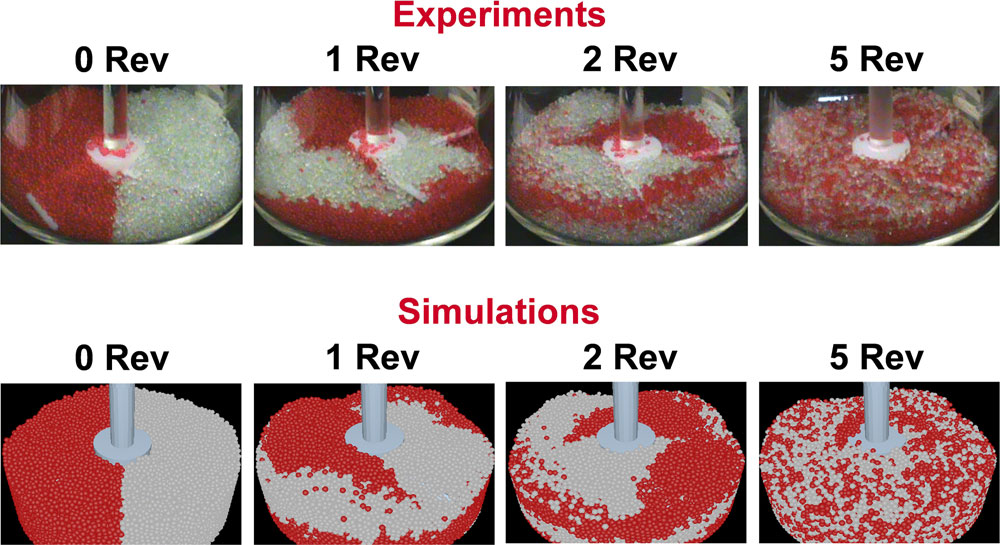
\includegraphics[width=0.65\textwidth]{images/introduction/drug_production.png}
% 	% {\centerline{\includegraphics[scale=#2]{#1}}}
% 	% \vspace{-0.2cm}
% 	\label{fig:verlet_distance}
% 	\source{\alert{Citar fonte}}
% 	% \vspace{-1cm}
% \end{figure}

% Para partículas esféricas \(\particlei\) e \(\particlej\), a condição de vizinhança se escreve como
% \begin{equation*}
% 	\norm{\positioni - \positionj} < \radiusi + \radiusj + \verletDistance,
% \end{equation*}
% como indicado na figura \ref{fig:verlet_distance}. Com isso, define-se a lista de Verlet da partícula \(i\) como
% \begin{equation*}
% 	\verletList[i] = \set{\elementj\in\elementSet\suchThat \norm{\positioni - \positionj} < \radiusi + \radiusj + \verletDistance}.
% \end{equation*}

% As listas de Verlet são construídas, para cada partícula, no início da simulação. Com a evolução do tempo, porém, a movimentação das partículas faz com que sua vizinhança se altere, e então é necessário reconstruir as listas. O critério para essa reconstrução leva em consideração a situação extrema em que duas partículas quase vizinhas tenham um deslocamento igual à metade da distância de Verlet uma em direção à outra, iniciando uma colisão. Para isso, define-se, para cada partícula, a posição de referência \(\verletPosition\) como a posição da partícula no momento em que as listas foram construídas. Tão logo a partícula se afaste dessa posição em uma distância igual à metade da distância de Verlet, as listas devem ser reconstruídas.

% Esse algoritmo pode ser implementado como na \cref{lst:verlet_list}

% \begin{lstlisting}[float, floatplacement=h, language=pseudocode, label=lst:verlet_list, caption=Pseudocódigo para a implementação das listas de Verlet.]
% // Definição da função de construção das listas de Verlet
% função "construir listas de Verlet":
% (*\indentrule*)	para cada partícula $\particlei\in\particleSet$:
% (*\indentrule*)	(*\indentrule*) atribuir $\verletPosition[i] \gets \positioni$
% (*\indentrule*)	(*\indentrule*)	inicializar $\verletList[i]$ como uma lista vazia
% (*\indentrule*)	(*\indentrule*)	para cada elemento $\elementj\in\elementSet$:
% (*\indentrule*)	(*\indentrule*)	(*\indentrule*)	se $\norm{\positioni - \positionj} < \radiusi + \radiusj + \verletDistance$:
% (*\indentrule*)	(*\indentrule*)	(*\indentrule*)	(*\indentrule*)	incluir $\elementj$ em $\verletList[i]$
% (*\indentrule*)	(*\indentrule*)	(*\indentrule*)	fim
% (*\indentrule*)	(*\indentrule*)	fim
% (*\indentrule*)	fim
% fim
% (*\hiddenCode*)
% chamar função  "construir listas de Verlet"
% enquanto o critério de parada não for atingido:
% (*\indentrule*)	(*\hiddenCode*) // Exportação de dados
% (*\indentrule*)	se $\norm{\positioni-\verletPosition[i]} \geq \bigslant{\verletDistance}{2}$ para alguma partícula ${}\particlei\in\particleSet$:
% (*\indentrule*)	(*\indentrule*)	chamar função  "construir listas de Verlet"
% (*\indentrule*)	fim
% (*\indentrule*)	(*\hiddenCode*) // Solução das equações
% fim
% \end{lstlisting}

% O algoritmo de Verlet, embora bastante eficiente para partículas esféricas, complica-se para o caso de partículas de geometria arbitrária, dada a necessidade de se conhecer sua a superfície.

% \subsection{Volume Envolvente}

% \subsection{Vizinhança Global}
% \subsection{Algoritmo \textit{link cell}}
% \subsection{Algoritmo \textit{lattice}}

% \subsection{Identificação de Contatos}

% \alert{Será necessária esta seção? Ela pode estar incluída no monitoramento de vizinhanças}

\section{Limitação do Passo de Tempo}

Diversos autores sugerem a limitação do passo de tempo da simulação para se garantirem a estabilidade numérica e a representatividade das soluções. Segundo \citeonline{bib:gomes2014}, uma estratégia possível é definir-se um valor de \textit{passo de tempo crítico} \(\criticalDt\) com a forma
\begin{equation} \label{eq:critical_dt}
	\criticalDt = C\cdot\sqrt{\bigslant{\mass}{\effectiveNormalElastic}},\quad C\in\real,
\end{equation}
sendo \(\mass\) a massa efetiva e \(\effectiveNormalElastic\) a constante elástica efetiva dos pares de colisão. O valor da constante \(C\) é, geralmente, determinado com base na experiência do usuário.

A limitação do passo de tempo, porém, depende fortemente da configuração da simulação. Por exemplo, quanto maiores forem as velocidades das partículas, menores os passos de tempo que devem ser usados a fim de evitar que as partículas se atravessem sem que a sua colisão seja computada. Entretanto a expressão em \eqref{eq:critical_dt} não indica nenhuma dependência com relação à velocidade.

Na ausência de melhores formulações, passos de tempo arbitrados acabam sendo utilizados nas simulações, e sua obtenção baseia-se fortemente na intuição do usuário, em cálculos prévios e na experimenação numérica.

\section{Condições de Contorno e Restrições} \label{sec:boundary_condition}

Comumente, além das interações entre partículas, os métodos de elementos discretos contam com condições adicionais para a execução das simulações. Essas considerações são denominadas de \textit{condições de contorno}. Dentre elas, as mais utilizadas são:
\begin{alineas}
\item \textit{Movimento prescrito:} circunstância em que o movimento de um elemento é totalmente determinado por uma função fornecida na etapa de inicialização. É essa a condição que rege os elementos de contorno.
\item \textit{Condição de repetição:} nesse caso, repete-se periodicamente a região da simulação em uma ou mais dimensões \cite[p. 15]{bib:computational_granular_dynamics}. Partículas que saem da região da simulação por um lado são reinseridas no lado oposto. Dessa forma, o domínio da simulação torna-se efetivamente infinito. A vizinhança de uma partícula deve, então, levar em consideração não apenas os elementos fisicamente próximos a ela, mas também aqueles localizados no extremo oposto da região de simulação, com os quais a partícula pode vir a colidir se houver o cruzamento das fronteiras. Mais detalhes sobre essa condição são apresentados por \citeonline[p. 24]{bib:liquids}, \citeonline{bib:bicanic2007} e \citeonline[p. 15]{bib:computational_granular_dynamics}.
\item \textit{Condição de reflexão:} essa condição resume-se à definição de paredes reflexivas. Quando uma partícula colide com um elemento desse tipo, sua velocidade é refletida com relação à parede, enquanto a componente de velocidade paralela à parede mantém-se inalterada, como representado na \cref{fig:boundary_conditions:reflecting_boundary}. Mais considerações acerca dessa condição podem ser encontradas em \citeonline[p. 169]{bib:computational_granular_dynamics}.

\begin{figure}[h]
	\caption{Restrição de movimento pela ação de molas aos subelementos de uma partícula composta.}
	% \vspace{-0.5cm}
	\centering
		\alert{Colocar imagem}
		% 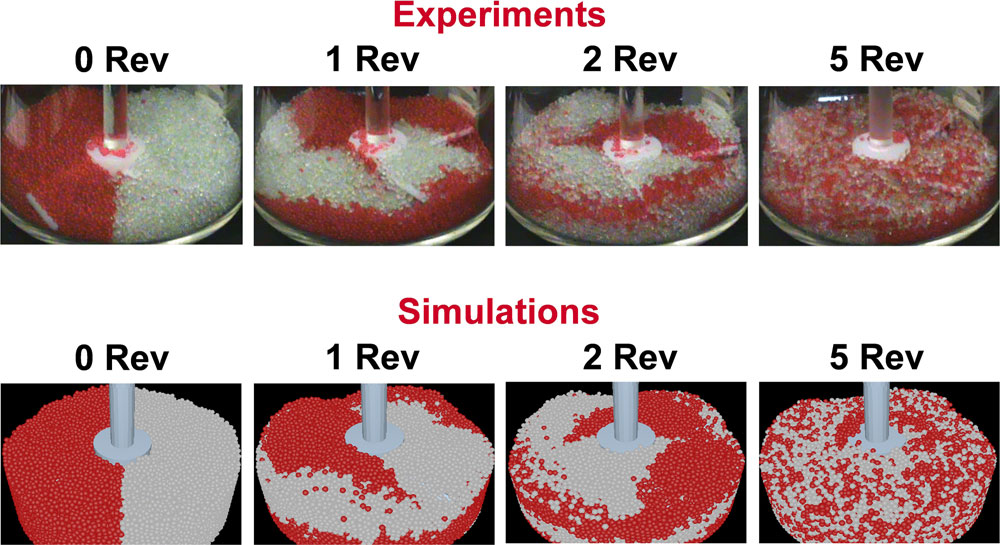
\includegraphics[width=0.65\textwidth]{images/introduction/drug_production.png}
	% {\centerline{\includegraphics[scale=#2]{#1}}}
	% \vspace{-0.2cm}
	\label{fig:boundary_conditions:reflecting_boundary}
	\source{\alert{Citar fonte}}
	% \vspace{-1cm}
\end{figure}

\item \textit{Restrição de movimento:} a restrição de movimento consiste em se acoplarem as equações de movimento de duas ou mais partículas. Essa condição encontra-se presente em partículas compostas para mediar a movimentação relativa entre os subelementos. Uma maneira simples de se implementar essa restrição é com a adição de uma força elástica representada pela ação de molas, como indicado na \cref{fig:boundary_conditions:restrition}.

\begin{figure}[h]
	\caption{Restrição de movimento pela ação de molas aos subelementos de uma partícula composta.}
	% \vspace{-0.5cm}
	\centering
		\alert{Colocar imagem}
		% 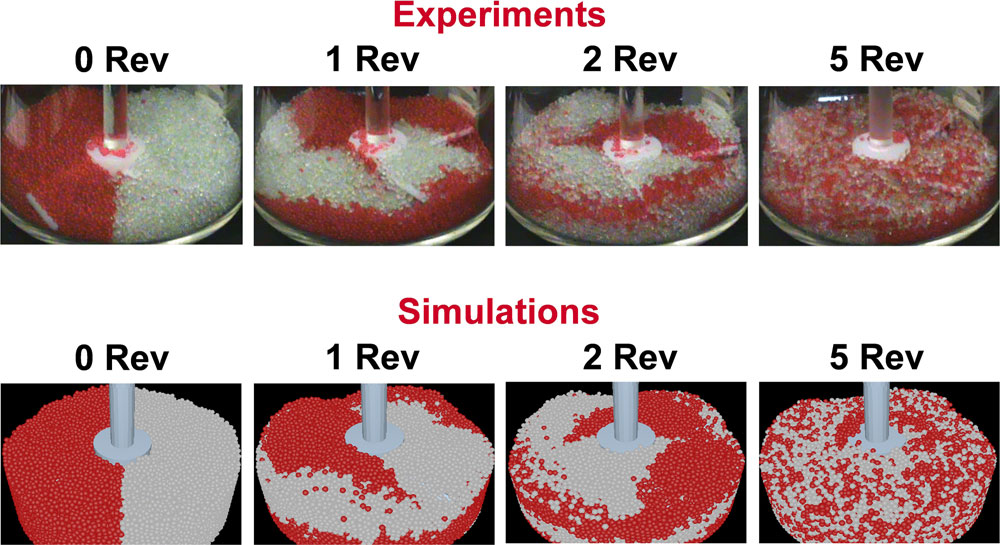
\includegraphics[width=0.65\textwidth]{images/introduction/drug_production.png}
	% {\centerline{\includegraphics[scale=#2]{#1}}}
	% \vspace{-0.2cm}
	\label{fig:boundary_conditions:restrition}
	\source{\alert{Citar fonte}}
	% \vspace{-1cm}
\end{figure}
\end{alineas}

\section{Outros Aspectos do Método}
\alert{Considerar, principalmente, \citeonline{bib:bicanic2007}. Essa seção deve falar que existem o estudo de fratura e fragmentação, abordagem para corpos deformáveis e esquemas de variação do passo de tempo}
\alert{Falar da paralelização}

\section{Acoplamento com Outros Métodos}
\alert{Falar aqui como o \DEM{} pode ser acoplado com CFD e FEM}